\section{ROS} \label{sec:ros}
ROS provee los servicios estándar de un sistema operativo tales como abstracción del hardware, control de dispositivos de bajo nivel, implementación de funcionalidad de uso común, paso de mensajes entre procesos y mantenimiento de paquetes.
\begin{figure}[h]
	\centering
	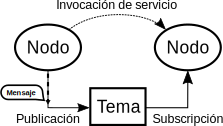
\includegraphics[width=0.5\linewidth]{img/ROS_concepts}
	\caption{Diagrama de comunicación de ROS}
	\label{fig:rosconcepts}
\end{figure}

Según \cite{ubuntuROS} asi está definido lo que es ROS.

\subsection{Nodo (Node)}

En ROS (Robot Operating System), un \textbf{nodo} es una unidad de procesamiento que ejecuta una función específica del sistema robótico. Los nodos pueden publicar información, suscribirse a otros nodos, o bien intercambiar información a través de servicios.

Aqui en \cite{rosNodeRoboticsBackend} se define lo que es un nodo.

\subsection{Tema (Topic)}

Un \textbf{tema} es un canal de comunicación utilizado para el envío de datos entre nodos de forma asincrónica. Un nodo puede publicar mensajes en un tema, mientras que otros nodos pueden suscribirse a ese tema para recibir los datos. Esta es la forma más común de comunicación en ROS.
 
 
\begin{itemize}
	\item \textbf{Publicador:} nodo que envía datos a un tema.
	\item \textbf{Suscriptor:} nodo que recibe datos de un tema.
\end{itemize}


\subsection{Mensaje (Message)}

Los \textbf{mensajes} son estructuras de datos estandarizadas que se transmiten a través de los temas. Pueden incluir tipos de datos como enteros, flotantes, vectores, matrices, imágenes, etc. Los tipos de mensajes están predefinidos en ROS y se agrupan por paquetes, como \texttt{std\_msgs}, \texttt{sensor\_msgs}, \texttt{geometry\_msgs}, entre otros.


\subsection{Servicio (Service)}

Un \textbf{servicio} en ROS es una forma de comunicación sincrónica que sigue el modelo de cliente-servidor. Un nodo ofrece un servicio y otro nodo lo invoca. La comunicación ocurre mediante una solicitud y una respuesta. Los servicios se usan cuando se necesita una operación puntual y no continua.


\begin{itemize}
	\item \textbf{Cliente:} nodo que solicita el servicio.
	\item \textbf{Servidor:} nodo que responde a la solicitud.
\end{itemize}


\subsection{Gazebo}


\textbf{Gazebo} es un simulador 3D que permite probar robots en entornos virtuales realistas. Se integra con ROS para simular sensores, actuadores, objetos y dinámicas físicas. Gazebo actúa como un nodo que publica datos (como imágenes de cámaras, posiciones, fuerzas) en temas de ROS, permitiendo desarrollar algoritmos sin usar hardware real.

En \cite{gazeboTheConstruct} se define Gazebo.

\subsection{RViz}

\textbf{RViz} (ROS Visualization) es una herramienta de visualización para ROS que permite observar el estado del robot, sus sensores y el entorno en un espacio tridimensional. Se suscribe a diversos temas del sistema y muestra información como:


\begin{itemize}
	\item Modelos del robot.
	\item Datos de sensores (cámaras, LIDAR).
	\item Trayectorias y mapas.
	\item Marcos de referencia (TF).
\end{itemize}


\subsection*{Resumen}
\begin{table}[H]
	\centering
	\begin{tabular}{|l|p{10cm}|}
		\hline
		\textbf{Elemento} & \textbf{Descripción} \\
		\hline
		Nodo & Proceso que realiza una tarea específica (ej. lectura de sensor, control de motor). \\
		Tema & Canal de comunicación asincrónico entre nodos. \\
		Mensaje & Estructura de datos que se transmite mediante un tema. \\
		Servicio & Comunicación sincrónica mediante solicitud y respuesta. \\
		Gazebo & Simulador físico 3D que emite datos hacia ROS. \\
		RViz & Visualizador 3D de datos del robot en tiempo real. \\
		\hline
	\end{tabular}
	\caption{Resumen de elementos clave en la comunicación de ROS}
\end{table}
